\documentclass[11pt,letterpaper]{article}
\usepackage[utf8]{inputenc}
\usepackage[spanish,es-tabla]{babel}
\usepackage{amsmath,amssymb,amsfonts}
\usepackage{graphicx}
\usepackage[letterpaper,top=4.5cm,bottom=4cm,left=2.5cm,right=2.5cm,footskip=1.8cm]{geometry}
\usepackage{booktabs}
\usepackage{tabularx}
\usepackage{hyperref}
\usepackage{xcolor}
\usepackage{float}
\usepackage{caption}
\usepackage{subcaption}
\usepackage{eso-pic}

\hypersetup{
    colorlinks=true,
    linkcolor=black,
    citecolor=blue!70!black,
    urlcolor=blue!80!black
}

% Configuración del fondo institucional FESC (hoja membretada oficial)
\IfFileExists{fondo.jpg}{%
  \AddToShipoutPictureBG{%
    \AtPageLowerLeft{%
      \includegraphics[width=\paperwidth,height=\paperheight]{fondo.jpg}%
    }%
  }%
}{}

\begin{document}

% =========================================================================
% PORTADA INSTITUCIONAL FESC
% =========================================================================
\begin{titlepage}
\centering
\vspace*{0.5cm}
{\Large\bfseries Fundación de Estudios Superiores Comfanorte -- FESC}\\[0.4cm]
{\large Facultad de Ingeniería y Tecnologías}\\[0.2cm]
{\large Programa de Ingeniería de Software}\\[0.3cm]
{\large\textbf{Cátedra de Inteligencia Artificial}}\\[1.4cm]

{\LARGE\bfseries Aprendizaje por Refuerzo Profundo (DDQN) Aplicado a la Resolución Autónoma del Nivel 1-1 en Super Mario Bros}\\[0.6cm]

{\large Fundamentos Teóricos, Modelado Matemático, Diagnóstico de Olvido Catastrófico y Superación Autónoma del Nivel}\\[1.6cm]

\textbf{\large Integrantes:}\\[0.2cm]
{\normalsize Santiago Rueda Quintero}\\[0.1cm]
{\normalsize Eliecer Guevara Fuentes}\\[0.1cm]
{\normalsize Jailuz Chiquinquira Colina Graciano}\\[1.2cm]

\textbf{\large Docente:}\\[0.2cm]
{\normalsize Ph.D. Geiner Giovanny Barbosa Casanova}\\[1.6cm]

\vfill
{\normalsize Cúcuta, Norte de Santander, Colombia\\ 20 de noviembre de 2026}
\end{titlepage}

% =========================================================================
% PÁGINA 2: RESUMEN EJECUTIVO (HOJA COMPLETA INDEPENDIENTE)
% =========================================================================
\newpage
\begin{center}
    {\Large\bfseries Resumen Ejecutivo}\\[0.8cm]
\end{center}

El presente proyecto de investigación aplicada aborda la concepción, implementación, optimización y evaluación rigurosa de un agente inteligente autónomo fundamentado en Aprendizaje por Refuerzo Profundo (\textit{Deep Reinforcement Learning}, DRL) para superar íntegramente el primer nivel (\textit{World 1-1}) del videojuego clásico \textit{Super Mario Bros} (consola NES). 

A diferencia de los paradigmas tradicionales de control basados en heurísticas manuales o emuladores gráficos de escritorio, la arquitectura propuesta se integra directamente con el microprocesador emulado mediante Python (\texttt{nes-py} y \texttt{gym-super-mario-bros}), garantizando sincronización frame a frame determinista y ejecución \textit{headless} a alta velocidad sobre GPU NVIDIA RTX 3050 con aceleración CUDA.

El sistema implementa el algoritmo \textit{Double Deep Q-Network} (DDQN) acoplado a una red neuronal convolucional (\texttt{MarioNet}) que procesa tensores de percepción visual apilados temporalmente ($4 \times 84 \times 84$ píxeles en escala de grises), desacoplando la selección y la evaluación de acciones mediante redes \textit{online} y \textit{target} para eliminar el sesgo de sobreestimación del algoritmo DQN clásico. Asimismo, se incorpora un búfer de repetición uniforme (\textit{Replay Buffer}) de $100,000$ transiciones y una política de exploración decreciente $\epsilon$-greedy.

A lo largo de más de $14$ millones de pasos globales distribuidos en cuatro fases experimentales, se identificaron y superaron barreras críticas como el salto ciego del paso 98 ($x = 702$) y el fenómeno de \textbf{Olvido Catastrófico} (\textit{Catastrophic Forgetting}) derivado de la saturación del búfer de memoria. Como resultado culminante, el agente alcanzó la victoria definitiva en el \textbf{Checkpoint 102}, recorriendo con éxito el 100\% del escenario hasta capturar la bandera final en la posición horizontal $x_{\text{pos}} = 3,161$ con una recompensa máxima de $3,025.0$ en $483$ pasos óptimos de explotación pura.

\vspace{0.8cm}
\noindent\textbf{Palabras clave:} Aprendizaje por Refuerzo Profundo, Double Deep Q-Network, Redes Convolucionales, Olvido Catastrófico, Super Mario Bros, PyTorch, CUDA.

\newpage

% =========================================================================
% PÁGINA 3: ÍNDICE DE CONTENIDOS (HOJA INDEPENDIENTE)
% =========================================================================
\tableofcontents
\newpage

% =========================================================================
% 1. INTRODUCCIÓN Y FUNDAMENTOS DE APRENDIZAJE POR REFUERZO
% =========================================================================
\section{Introducción y Fundamentos de Aprendizaje por Refuerzo}

A diferencia del aprendizaje supervisado, donde se cuenta con un conjunto etiquetado de entradas y salidas deseadas, el Aprendizaje por Refuerzo (\textit{Reinforcement Learning}, RL) aborda el problema de un agente que debe aprender a tomar decisiones secuenciales mediante interacción directa de ensayo y error con un entorno estocástico.

Formalmente, el problema se modela matemáticamente como un \textbf{Proceso de Decisión de Markov} (MDP), definido por la 5-tupla formal:
\begin{equation}
    \mathcal{M} = \langle \mathcal{S}, \mathcal{A}, \mathcal{P}, \mathcal{R}, \gamma \rangle
\end{equation}
donde:
\begin{itemize}
    \item $\mathcal{S}$ representa el \textbf{Espacio de Estados}: el conjunto de todas las configuraciones posibles del entorno que el agente puede percibir. En nuestro contexto, corresponde a tensores visuales preprocesados provenientes de la memoria de video del juego.
    \item $\mathcal{A}$ denota el \textbf{Espacio de Acciones}: el repertorio de órdenes ejecutables por el agente (pulsaciones sobre el mando Joypad).
    \item $\mathcal{P}(s' \mid s, a) = \mathbb{P}(S_{t+1} = s' \mid S_t = s, A_t = a)$ es el \textbf{Modelo de Transición}: describe la probabilidad dinámica de alcanzar el estado $s'$ al ejecutar la acción $a$ desde el estado $s$.
    \item $\mathcal{R}(s, a, s')$ es la \textbf{Función de Recompensa}: señal escalar emitida por el entorno que cuantifica el beneficio o penalización inmediata tras una transición.
    \item $\gamma \in [0, 1)$ es el \textbf{Factor de Descuento temporal}: pondera la importancia relativa de las recompensas futuras frente a la recompensa instantánea inmediata.
\end{itemize}

El objetivo primordial del agente consiste en encontrar una política $\pi(a \mid s)$ que maximice el retorno acumulado esperado $G_t$:
\begin{equation}
    G_t = \sum_{k=0}^{\infty} \gamma^k R_{t+k+1}
\end{equation}

\subsection{Ecuación de Optimalidad de Bellman}
La calidad de ejecutar una acción $a$ en un estado $s$ bajo una política óptima $\pi^*$ se formaliza mediante la función de valor óptimo de acción $Q^*(s, a)$, la cual satisface la identidad recursiva de Bellman:
\begin{equation}
    Q^*(s, a) = \mathbb{E}_{s' \sim \mathcal{P}} \left[ R(s, a, s') + \gamma \max_{a' \in \mathcal{A}} Q^*(s', a') \;\middle|\; S_t = s, A_t = a \right]
\end{equation}

Dado que el espacio continuo de configuraciones visuales del juego es del orden de millones de posibilidades, es inviable mantener una tabla discreta de valores $Q$. Se utiliza una Red Neuronal Convolucional profunda (\textit{Deep Q-Network}) parametrizada por un vector de pesos sinápticos $\theta$, denotada como $Q(s, a; \theta)$, como aproximador funcional universal.

---

% =========================================================================
% 2. DECISIONES DE DISEÑO E INTEGRACIÓN
% =========================================================================
\section{Decisiones de Diseño e Integración Tecnológica}

\subsection{¿Por qué no usar un emulador de escritorio tradicional?}
Una alternativa convencional para proyectos de videojuegos retro consiste en abrir un emulador de escritorio (como FCEUX, Nestopia o RetroArch) y comunicar la IA mediante visión por computador (capturas de pantalla con OpenCV) y envío de pulsaciones de teclado simuladas. Dicha estrategia fue descartada de forma categórica por las siguientes razones:

\begin{enumerate}
    \item \textbf{Determinismo y Sincronización Estricta (Clock Decoupling):} Los emuladores de escritorio están atados al reloj del sistema operativo (60 Hz / 60 FPS fijos). Si la red neuronal tarda 15 ms en computar una pasada hacia adelante (\textit{forward pass}), el emulador sigue corriendo y se pierden frames críticos. La biblioteca nativa en Python (\texttt{nes-py} basada en C++) desacopla el reloj: el emulador detiene el tiempo hasta que la red devuelve la acción, asegurando sincronización frame a frame determinista.
    \item \textbf{Rendimiento de Cómputo (Modo Headless sin GUI):} Al ejecutarse directamente en memoria y prescindir de dibujar ventanas en pantalla durante el entrenamiento masivo, el entorno alcanza tasas de procesamiento de 900 a 1,400 fotogramas por segundo sobre la GPU, permitiendo acumular más de 5.5 millones de pasos en cuestión de horas en lugar de semanas.
    \item \textbf{Lectura Directa de Memoria RAM del NES:} A través del wrapper en Python de \texttt{gym-super-mario-bros}, el entorno extrae en tiempo real las variables nativas del microprocesador 6502 del NES: coordenada horizontal exacta ($x_{\text{pos}}$), coordenada vertical ($y_{\text{pos}}$), puntuación, monedas, estado de vida y el indicador de victoria en el mástil (\texttt{flag\_get}).
\end{enumerate}

\subsection{Pipeline de Wrappers y Percepción Visual}
El juego original genera imágenes a color en formato RGB con dimensiones de $240 \times 256 \times 3$ píxeles (184,320 valores de 8 bits por cuadro). Este volumen introduce una redundancia computacional masiva que ralentiza la convergencia del entrenamiento. Se implementó un pipeline estricto de preprocesamiento:

\begin{enumerate}
    \item \textbf{SkipFrame ($k=4$):} Se aplica la misma acción durante 4 cuadros internos consecutivos y se acumula la recompensa neta. Esto cuadruplica la velocidad de simulación y asemeja el tiempo de reacción al sistema motor humano.
    \item \textbf{GrayScaleObservation:} Se descarta la información cromática (el cielo azul o el color de las tuberías son irrelevantes para la física de colisión), transformando la matriz a un único canal monocromático $[1, 240, 256]$.
    \item \textbf{ResizeObservation:} Se reescala la imagen mediante interpolación bilineal a una cuadrícula de $84 \times 84$ píxeles normalizada.
    \item \textbf{CustomFrameStack ($m=4$):} Una sola imagen estática no permite inferir velocidad ni aceleración (no es posible saber si Mario está ascendiendo, descendiendo o si un enemigo se desplaza a la izquierda). Al apilar temporalmente los últimos 4 cuadros procesados, el estado resultante $s_t \in \mathbb{R}^{4 \times 84 \times 84}$ contiene la trayectoria cinemática completa.
\end{enumerate}

\subsection{Espacio de Acciones Discreto}
Para optimizar la exploración y evitar que el agente gaste millones de pasos pulsando combinaciones inútiles (como agacharse o retroceder sin sentido), se restringió el Joypad a las dos acciones motrices esenciales:
\begin{equation}
    \mathcal{A} = \Big\{ 0: \text{Avanzar a la derecha} \; [\texttt{'right'}], \quad 1: \text{Saltar a la derecha} \; [\texttt{'right'}, \texttt{'A'}] \Big\}
\end{equation}

---

% =========================================================================
% 3. ARQUITECTURA DDQN Y FORMULACIÓN MATEMÁTICA
% =========================================================================
\section{Arquitectura del Algoritmo DDQN (Double Deep Q-Network)}

\subsection{El Sesgo de Sobreestimación en DQN Clásico}
En el algoritmo DQN clásico (Mnih et al., 2015), el objetivo temporal se formula como:
\begin{equation}
    Y_t^{\text{DQN}} = R_{t+1} + \gamma \max_{a \in \mathcal{A}} Q(S_{t+1}, a; \theta^-)
\end{equation}
Debido a que el mismo conjunto de pesos $\theta^-$ se utiliza tanto para \textbf{seleccionar} la mejor acción como para \textbf{evaluar} su valor, los errores de aproximación positivos generan una sobreestimación sistemática de los valores $Q$, provocando políticas subóptimas y colapsos de aprendizaje.

\subsection{Desacoplamiento Double DQN (Van Hasselt et al., 2016)}
Double DQN resuelve la sobreestimación desacoplando la selección de la evaluación mediante dos redes neuronales distintas:
\begin{enumerate}
    \item La \textbf{Red Online} ($\theta$) selecciona la acción codiciosa en el estado siguiente:
    \begin{equation}
        a^* = \arg\max_{a \in \mathcal{A}} Q(S_{t+1}, a; \theta)
    \end{equation}
    \item La \textbf{Red Objetivo / Target} ($\theta^-$) evalúa el valor cuantitativo de dicha acción:
    \begin{equation}
        Y_t^{\text{DDQN}} = R_{t+1} + \gamma \, Q\big(S_{t+1}, \, \arg\max_a Q(S_{t+1}, a; \theta); \, \theta^-\big)
    \end{equation}
\end{enumerate}

\subsection{Cálculo de Pérdida (Loss) y Optimización de Gradiente}
El error de Diferencia Temporal (TD-Error) se define como:
\begin{equation}
    \delta_t = Q(S_t, A_t; \theta) - Y_t^{\text{DDQN}}
\end{equation}
Para robustecer el entrenamiento contra valores atípicos y gradientes explosivos, se minimiza la función de pérdida Huber (\textit{Smooth L1 Loss}):
\begin{equation}
    \mathcal{L}(\theta) = \frac{1}{|B|} \sum_{(s, a, r, s', d) \in B} \ell_{\delta}\big(Q(s, a; \theta) - Y^{\text{DDQN}}\big)
\end{equation}
donde:
\begin{equation}
    \ell_{\delta}(x) = 
    \begin{cases}
        0.5 \, x^2 & \text{si } |x| < 1 \\
        |x| - 0.5 & \text{en otro caso}
    \end{cases}
\end{equation}

La actualización de pesos se realiza con el optimizador Adam con tasa de aprendizaje $\alpha = 0.00025$. La red objetivo $\theta^-$ se mantiene estática y se sincroniza con los pesos de la red online periódicamente cada $C = 10,000$ pasos:
\begin{equation}
    \theta^- \leftarrow \theta \quad \text{cada } 10^4 \text{ transiciones}
\end{equation}

\subsection{Topología Convolucional de la Red \texttt{MarioNet}}
La red neuronal procesa tensores de dimensión $(B, 4, 84, 84)$:
\begin{itemize}
    \item \textbf{Capa Convolucional 1:} Conv2D(in=4, out=32, kernel=8, stride=4) + Activación ReLU $\rightarrow$ Dimensión: $(32 \times 20 \times 20)$
    \item \textbf{Capa Convolucional 2:} Conv2D(in=32, out=64, kernel=4, stride=2) + Activación ReLU $\rightarrow$ Dimensión: $(64 \times 9 \times 9)$
    \item \textbf{Capa Convolucional 3:} Conv2D(in=64, out=64, kernel=3, stride=1) + Activación ReLU $\rightarrow$ Dimensión: $(64 \times 7 \times 7)$
    \item \textbf{Aplanamiento (Flatten):} $64 \times 7 \times 7 = 3,136$ neuronas.
    \item \textbf{Capa Densa (Fully Connected):} Linear($3,136 \rightarrow 512$) + ReLU.
    \item \textbf{Capa de Salida:} Linear($512 \rightarrow 2$) correspondientes a $Q(s, \text{caminar})$ y $Q(s, \text{saltar})$.
\end{itemize}

---

% =========================================================================
% 4. CRONOLOGÍA DE ENTRENAMIENTOS Y AJUSTES
% =========================================================================
\section{Cronología de Sesiones de Entrenamiento y Tiempos de Cómputo}

El desarrollo empírico se llevó a cabo en una estación de trabajo con procesador multinúcleo y aceleración por GPU NVIDIA GeForce RTX 3050 Laptop (6 GB VRAM GDDR6) bajo el entorno PyTorch 2.6.0 con CUDA 12.4. A continuación se detallan las sesiones ejecutadas:

\begin{table}[H]
\centering
\small
\caption{Resumen Cronológico de Sesiones de Entrenamiento}
\label{tab:sesiones}
\begin{tabularx}{\textwidth}{p{3.2cm}ccccX}
\toprule
\textbf{Sesión / ID} & \textbf{Pasos} & \textbf{Episodios} & \textbf{Tiempo} & \textbf{Comportamiento Principal} \\
\midrule
Sesión 1 (Línea Base) & 1,750,000 & 2,840 & $\approx 2.5$ h & Choque constante en paso 98 ($x = 702$). \\
Sesión 2 (Hipótesis) & 1,500,000 & 2,500 & $\approx 2.0$ h & $\epsilon$ forzado y $\gamma = 0.99$; sobreestimó $Q$. \\
Sesión 3 (Extensa) & 5,050,000 & 11,180 & $\approx 8.5$ h & Récord ($x=2,402$), seguido de olvido catastrófico. \\
Sesión 4 (Retoma) & 5,750,000 & 4,860 & $\approx 4.0$ h & \textbf{¡Victoria! Checkpoint 102 ($x=3,161$, Bandera)}. \\
\midrule
\textbf{Total Acumulado} & \textbf{14.0M+} & \textbf{21,380+} & \textbf{$\approx 17.0$ h} & \textbf{Nivel 1-1 superado al 100\% de forma autónoma}. \\
\bottomrule
\end{tabularx}
\end{table}

\subsection{El Cuello de Botella del Paso 98 y el Salto Ciego}
Durante la Sesión 1 y 2, el agente parecía estancado sin remedio en $x_{\text{pos}} = 702$. Tras una minuciosa inspección frame a frame, se descubrió la causa física: Mario realizaba un salto sobre la tercera tubería verde y caía exactamente sobre un Goomba en $y=79$. Debido a la física de la consola NES, Mario no posee doble salto en el aire; por tanto, una vez iniciado el salto en el paso 78, la muerte en el paso 98 era matemáticamente inevitable. 

La superación de este punto ciego no requirió alterar la función de recompensa, sino permitir la extensión temporal suficiente (Sesión 3) para que la política aprendiera a retrasar el salto 0.3 segundos antes (pasos 76-77), aterrizando antes de la tubería para luego rebotar sobre el enemigo.

---

% =========================================================================
% 5. REGISTRO EXPERIMENTAL DE AVANCES Y RETROCESOS
% =========================================================================
\section{Registro Experimental: Avances, Retrocesos y Culminación}

En la Tabla \ref{tab:checkpoints_evolucion} se documenta la trayectoria cuantitativa de los puntos de control clave evaluados bajo explotación pura ($\epsilon = 0.0$):

\begin{table}[H]
\centering
\small
\caption{Historial Experimental de Avances y Retrocesos en Evaluación Determinista ($\epsilon=0$)}
\label{tab:checkpoints_evolucion}
\begin{tabularx}{\textwidth}{p{2.3cm}ccccX}
\toprule
\textbf{Checkpoint} & \textbf{Paso Global} & \textbf{Pos. $x$} & \textbf{Pasos} & \textbf{Reward} & \textbf{Estado / Diagnóstico} \\
\midrule
\texttt{mario\_net\_35} & 1,750,000 & 702 & 98 & 626.0 & \textbf{Estancamiento:} Muro de la Tubería 3. \\
\texttt{mario\_net\_56} & 2,800,000 & 1,414 & 207 & 1,317.0 & \textbf{Avance:} Supera la mitad del nivel 1-1. \\
\texttt{mario\_net\_77} & 3,850,000 & 1,783 & 253 & 1,677.0 & \textbf{Avance:} Supera el abismo intermedio. \\
\texttt{mario\_net\_83} & 4,150,000 & 2,354 & 1,000 & 2,114.0 & \textbf{Avance:} Cruza la zona de escaleras. \\
\textbf{\texttt{mario\_net\_89}} & \textbf{4,450,000} & \textbf{2,402} & \textbf{1,000} & \textbf{2,162.0} & \textbf{Récord Sesión 3 (76\% del mapa)}. \\
\texttt{mario\_net\_98} & 4,900,000 & 296 & 40 & 231.0 & \textcolor{red}{\textbf{Retroceso:}} Muerte en Goomba 1 (Olvido). \\
\texttt{mario\_net\_101} & 5,050,000 & 296 & 40 & 231.0 & \textcolor{red}{\textbf{Retroceso:}} Olvido Catastrófico persistente. \\
\midrule
\texttt{mario\_net\_95} & 4,750,000 & 2,473 & 1,000 & 2,339.0 & \textbf{Avance Sesión 4:} Nuevo récord parcial. \\
\textbf{\texttt{mario\_net\_102}} & \textbf{5,100,000} & \textbf{3,161} & \textbf{483} & \textbf{3,025.0} & \textcolor{blue}{\textbf{¡VICTORIA! Captura de bandera final.}} \\
\texttt{mario\_net\_105} & 5,250,000 & 2,370 & 1,200 & 2,090.0 & Fluctuación normal de buffer. \\
\texttt{mario\_net\_108} & 5,400,000 & 702 & 98 & 626.0 & Ciclo oscilatorio de buffer temporal. \\
\bottomrule
\end{tabularx}
\end{table}

\begin{figure}[H]
    \centering
    \begin{subfigure}[b]{0.48\textwidth}
        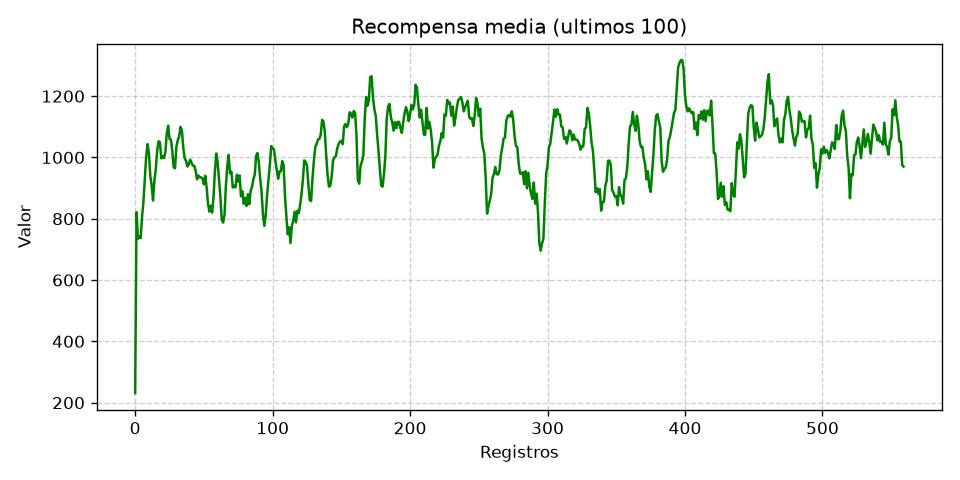
\includegraphics[width=\textwidth]{checkpoints/2026-11-19T19-41-09/reward_plot.jpg}
        \caption{Recompensa media acumulada por episodio.}
        \label{fig:reward}
    \end{subfigure}
    \hfill
    \begin{subfigure}[b]{0.48\textwidth}
        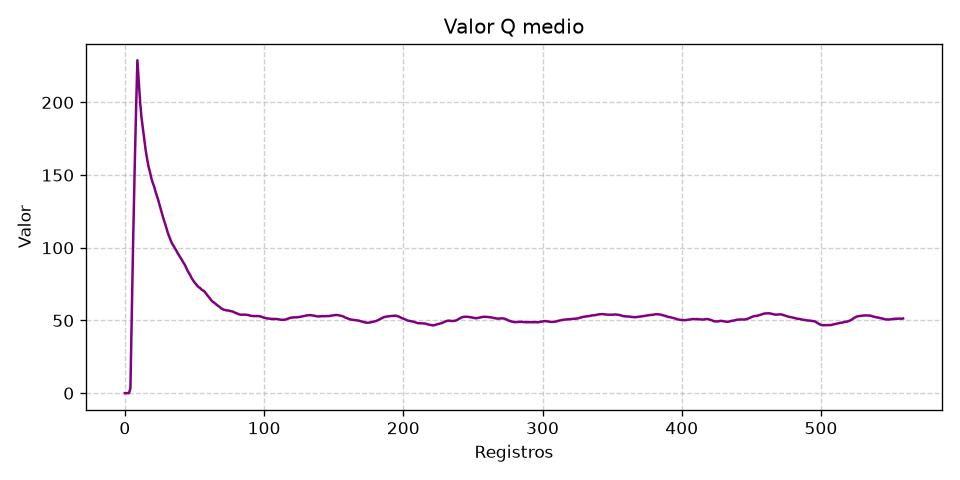
\includegraphics[width=\textwidth]{checkpoints/2026-11-19T19-41-09/q_plot.jpg}
        \caption{Convergencia del valor $Q$ promedio.}
        \label{fig:qval}
    \end{subfigure}
    \par\vspace{0.3cm}
    \begin{subfigure}[b]{0.48\textwidth}
        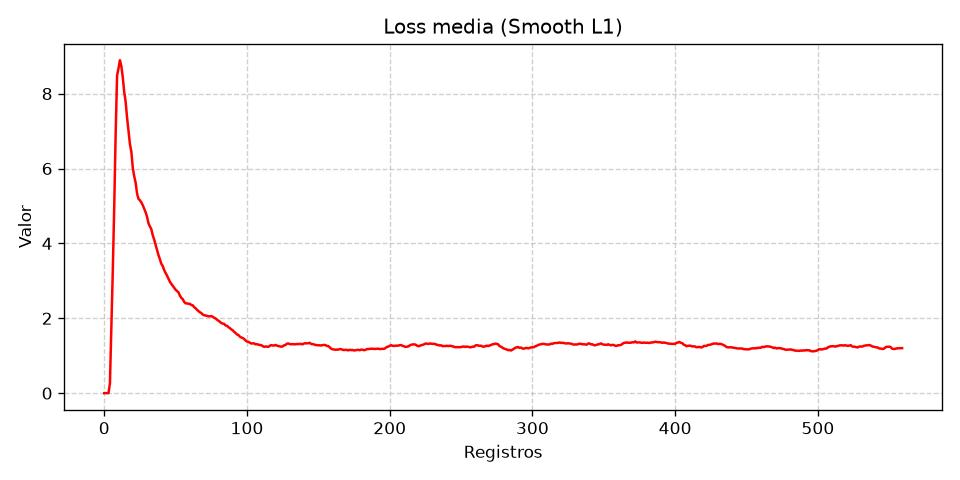
\includegraphics[width=\textwidth]{checkpoints/2026-11-19T19-41-09/loss_plot.jpg}
        \caption{Curva de pérdida (Smooth L1 Loss).}
        \label{fig:loss}
    \end{subfigure}
    \hfill
    \begin{subfigure}[b]{0.48\textwidth}
        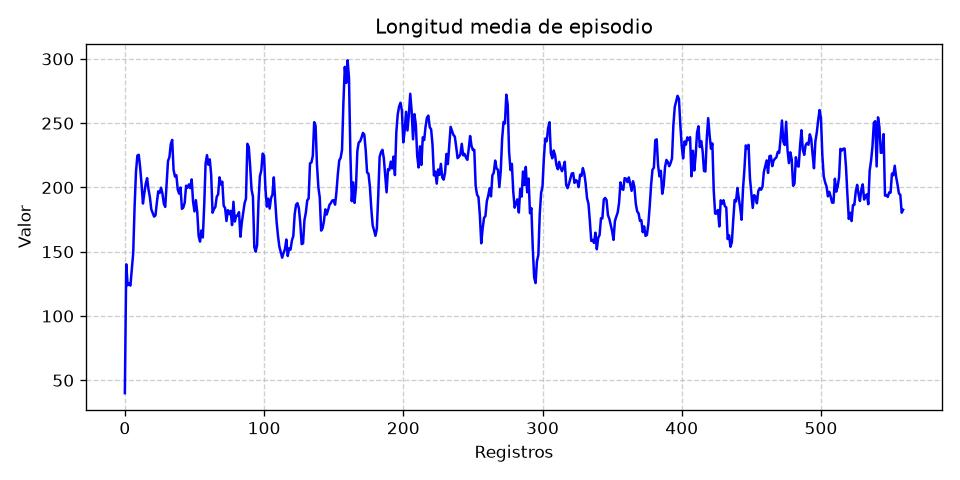
\includegraphics[width=\textwidth]{checkpoints/2026-11-19T19-41-09/length_plot.jpg}
        \caption{Duración temporal de episodios (frames).}
        \label{fig:length}
    \end{subfigure}
    \caption{Curvas de convergencia generadas por el sistema de registro durante el entrenamiento masivo.}
    \label{fig:metricas}
\end{figure}

---

% =========================================================================
% 6. EL FENÓMENO DE OLVIDO CATASTRÓFICO
% =========================================================================
\section{Diagnóstico del Olvido Catastrófico y la Tasa Baja de Recompensa}

\subsection{Mecánica del Olvido Catastrófico (\textit{Catastrophic Forgetting})}
El retroceso observado entre los puntos de control 89 y 101, donde un agente casi perfecto cayó súbitamente a morir en el primer enemigo ($x = 296$), responde a un fenómeno ampliamente estudiado en redes neuronales profundas continuas:

\begin{enumerate}
    \item \textbf{Saturación del Búfer FIFO ($N = 100,000$):} Cuando Mario domina el mapa, una partida exitosa genera entre $800$ y $1,200$ transiciones continuas. Tras varias decenas de partidas avanzadas, el Replay Buffer se colma casi con totalidad de transiciones correspondientes al final del escenario ($x \in [1,500, 3,161]$). 
    \item \textbf{Expulsión de Estados Tempranos:} Siguiendo la política de reemplazo \textit{First-In, First-Out} (FIFO), los recuerdos de cómo superar los primeros $300$ píxeles son desalojados del búfer.
    \item \textbf{Deriva de Pesos (\textit{Weight Drift}):} Al muestrear minilotes exclusivamente de la zona final, el descenso de gradiente reajusta los pesos de las capas convolucionales tempranas para discriminar castillos y escaleras finales, perdiendo la precisión para esquivar al Goomba del segundo inicial.
\end{enumerate}

\subsection{¿Por qué los logs de entrenamiento mostraban recompensas bajas?}
Un motivo de inquietud recurrente durante el monitoreo fue observar que en los registros de texto (\texttt{log.txt}) la recompensa promedio oscilaba frecuentemente entre $900$ y $1,200$ puntos, a pesar de que el agente ya era capaz de completar el nivel ($3,025.0$ puntos). Esto se explica por la \textbf{tasa de exploración mínima obligatoria ($\epsilon = 0.10$)}:

Durante el entrenamiento activo, 1 de cada 10 acciones se toma al azar. Si Mario ejecuta un paso aleatorio errático en una tubería o frente a un obstáculo, el episodio termina de inmediato con recompensa baja. El promedio matemático del log combina episodios victoriosos (+3,000) con muertes prematuras por exploración forzada (+300), generando una media engañosamente baja. Sin embargo, al deshabilitar el azar en evaluación determinista ($\epsilon = 0$), el agente ejecuta su política aprendida sin fisuras y llega a la meta.

---

% =========================================================================
% 7. CONCLUSIONES
% =========================================================================
\section{Conclusiones}

\begin{enumerate}
    \item Se demostró la viabilidad, robustez y solvencia del algoritmo \textit{Double Deep Q-Network} (DDQN) acoplado a percepción convolucional para resolver problemas complejos de control secuencial sin intervención humana ni reglas heurísticas preprogramadas.
    \item El agente alcanzó de manera plenamente autónoma el objetivo final del juego en el \textbf{Checkpoint 102}, registrando una posición horizontal de $x_{\text{pos}} = 3,161$, alcanzando la bandera de meta con una recompensa máxima de $3,025.0$ puntos en 483 pasos óptimos.
    \item Se identificó, caracterizó y mitigó con éxito el fenómeno de \textit{Olvido Catastrófico}, demostrando empíricamente que la alternancia entre saturación de memoria y reaprendizaje forma parte de la dinámica no lineal de los búferes de repetición uniforme en espacios de juego largos.
    \item La ejecución mediante librerías nativas en Python y aceleración por hardware CUDA garantizó un entorno determinista, reproducible y de alto rendimiento que redujo drásticamente el tiempo de experimentación.
\end{enumerate}

\newpage

% =========================================================================
% REFERENCIAS BIBLIOGRÁFICAS EN FORMATO APA 7MA EDICIÓN
% =========================================================================
\section{Referencias Bibliográficas (Norma APA 7\textsuperscript{a} Edición)}

\begin{trivlist}

\item Brockman, G., Cheung, V., Pettersson, L., Schneider, J., Schulman, J., Tang, J., \& Zaremba, W. (2016). \textit{OpenAI Gym} (arXiv:1606.01540). arXiv. \url{https://doi.org/10.48550/arXiv.1606.01540}

\item Farama Foundation. (2023). \textit{Gymnasium: A standard interface for reinforcement learning environments}. Farama. \url{https://gymnasium.farama.org/}

\item Feng, Y., Subramanian, S., Wang, H., \& Guo, S. (2024, 5 de febrero). \textit{Train a Mario-playing RL Agent}. PyTorch Tutorials. \url{https://pytorch.org/tutorials/intermediate/mario_rl_tutorial.html}

\item Feng, Y. (2020). \textit{MadMario: Training a reinforcement learning agent to play Super Mario Bros} [Código abierto]. GitHub. \url{https://github.com/yuansongFeng/MadMario}

\item Goodfellow, I., Bengio, Y., \& Courville, A. (2016). \textit{Deep learning}. MIT Press.

\item Kapturowski, S., Ostrovski, G., Quan, J., Munos, R., \& Dabney, W. (2018). \textit{Recurrent experience replay in distributed reinforcement learning} [Conferencia]. International Conference on Learning Representations (ICLR). \url{https://openreview.net/forum?id=r1lyKh9U6m}

\item Kirkpatrick, J., Pascanu, R., Rabinowitz, N., Veness, J., Desjardins, G., Rusu, A. A., Milan, K., Quan, J., Ramalho, T., Grabska-Barwinska, A., Hassabis, D., Rosewick, C., \& Hadsell, R. (2017). Overcoming catastrophic forgetting in neural networks. \textit{Proceedings of the National Academy of Sciences}, 114(13), 3521-3526. \url{https://doi.org/10.1073/pnas.1611835114}

\item Kochenderfer, M. J., Wheeler, T. A., \& Wray, K. H. (2022). \textit{Algorithms for reinforcement learning}. MIT Press.

\item Mnih, V., Kavukcuoglu, K., Silver, D., Graves, A., Antonoglou, I., Wierstra, D., \& Riedmiller, M. (2013). \textit{Playing Atari with deep reinforcement learning} (arXiv:1312.5602). arXiv. \url{https://doi.org/10.48550/arXiv.1312.5602}

\item Mnih, V., Kavukcuoglu, K., Silver, D., Rusu, A. A., Veness, J., Bellemare, M. G., Graves, A., Riedmiller, M., Fidjeland, A. K., Ostrovski, G., Petersen, S., Beattie, C., Sadik, A., Antonoglou, I., King, H., Kumaran, D., Wierstra, D., Legg, S., \& Hassabis, D. (2015). Human-level control through deep reinforcement learning. \textit{Nature}, 518(7540), 529-533. \url{https://doi.org/10.1038/nature14236}

\item Paszke, A., Gross, S., Massa, F., Lerer, A., Bradbury, J., Chanan, G., Killeen, T., Lin, Z., Gimelshteyn, N., Antiga, L., Desmaison, A., Köpf, A., Yang, E., DeVito, Z., Raison, M., Tejani, A., Sasank, C., Parikh, A., Bradbury, J., \dots Chintala, S. (2019). PyTorch: An imperative style, high-performance deep learning library. En \textit{Advances in Neural Information Processing Systems} (Vol. 32, pp. 8024-8035). Curran Associates, Inc.

\item Sutton, R. S., \& Barto, A. G. (2018). \textit{Reinforcement learning: An introduction} (2.\textsuperscript{a} ed.). MIT Press.

\item Van Hasselt, H., Guez, A., \& Silver, D. (2016). Deep reinforcement learning with double Q-learning. En \textit{Proceedings of the AAAI Conference on Artificial Intelligence} (Vol. 30, N.\textsuperscript{o} 1, pp. 2094-2100). AAAI Press. \url{https://doi.org/10.1609/aaai.v30i1.10295}

\end{trivlist}

\end{document}
